\documentclass{scaffold/sigchi}
\usepackage{pifont} % Check marks
\newcommand{\cmark}{\ding{51}} % So we can use \cmark instead of \ding{51}
\newcommand{\xmark}{\ding{55}}
%\usepackage[none]{hyphenat}


% Title
\def\plaintitle{Impact of Audio and Visual Display of Positive Reinforcement on Supporting Habit Formation}
%\def\plaintitle{Investigating the Impact of Displaying Positive Reinforcement Using Different Modalities on Habit Formation}

% Authors as plain text
\def\plainauthor{First Author, Second Author, Third Author,
  Fourth Author, Fifth Author, Sixth Author}
\def\emptyauthor{}
\def\plainkeywords{habit formation; behaviour change; positive reinforcement}
\def\plaingeneralterms{Documentation, Standardization}
  \usepackage{pgfplots}
  \pgfplotsset{compat=1.12}

% Use this section to set the ACM copyright statement (e.g. for
% preprints).  Consult the conference website for the camera-ready
% copyright statement.

% Copyright
\CopyrightYear{2017}
%\setcopyright{acmcopyright}
\setcopyright{acmlicensed}
%\setcopyright{rightsretained}
%\setcopyright{usgov}
%\setcopyright{usgovmixed}
%\setcopyright{cagov}
%\setcopyright{cagovmixed}
% DOI
\doi{http://dx.doi.org/10.475/123_4}
% ISBN
\isbn{123-4567-24-567/08/06}
%Conference
\conferenceinfo{CHI'18,}{April 21--26, 2018, Montreal, Canada}
%Price
% \acmPrice{\$15.00}

% Use this command to override the default ACM copyright statement
% (e.g. for preprints).  Consult the conference website for the
% camera-ready copyright statement.

%% HOW TO OVERRIDE THE DEFAULT COPYRIGHT STRIP --
%% Please note you need to make sure the copy for your specific
%% license is used here!
% \toappear{
% Permission to make digital or hard copies of all or part of this work
% for personal or classroom use is granted without fee provided that
% copies are not made or distributed for profit or commercial advantage
% and that copies bear this notice and the full citation on the first
% page. Copyrights for components of this work owned by others than ACM
% must be honored. Abstracting with credit is permitted. To copy
% otherwise, or republish, to post on servers or to redistribute to
% lists, requires prior specific permission and/or a fee. Request
% permissions from \href{mailto:Permissions@acm.org}{Permissions@acm.org}. \\
% \emph{CHI '16},  May 07--12, 2016, San Jose, CA, USA \\
% ACM xxx-x-xxxx-xxxx-x/xx/xx\ldots \$15.00 \\
% DOI: \url{http://dx.doi.org/xx.xxxx/xxxxxxx.xxxxxxx}
% }

% Arabic page numbers for submission.  Remove this line to eliminate
% page numbers for the camera ready copy
% \pagenumbering{arabic}

% Load basic packages
\usepackage{balance}       % to better equalize the last page
\usepackage{graphics}      % for EPS, load graphicx instead 
\usepackage[T1]{fontenc}   % for umlauts and other diaeresis
\usepackage{txfonts}
\usepackage{mathptmx}
\usepackage[pdflang={en-US},pdftex]{hyperref}
\usepackage{color}
\usepackage{booktabs}
\usepackage{textcomp}

% Some optional stuff you might like/need.
\usepackage{microtype}        % Improved Tracking and Kerning
% \usepackage[all]{hypcap}    % Fixes bug in hyperref caption linking
\usepackage{ccicons}          % Cite your images correctly!
% \usepackage[utf8]{inputenc} % for a UTF8 editor only

% If you want to use todo notes, marginpars etc. during creation of
% your draft document, you have to enable the "chi_draft" option for
% the document class. To do this, change the very first line to:
% "\documentclass[chi_draft]{sigchi}". You can then place todo notes
% by using the "\todo{...}"  command. Make sure to disable the draft
% option again before submitting your final document.
\usepackage{todonotes}






% llt: Define a global style for URLs, rather that the default one
\makeatletter
\def\url@leostyle{%
  \@ifundefined{selectfont}{
    \def\UrlFont{\sf}
  }{
    \def\UrlFont{\small\bf\ttfamily}
  }}
\makeatother
\urlstyle{leo}




% To make various LaTeX processors do the right thing with page size.
\def\pprw{8.5in}
\def\pprh{11in}
\special{papersize=\pprw,\pprh}
\setlength{\paperwidth}{\pprw}
\setlength{\paperheight}{\pprh}
\setlength{\pdfpagewidth}{\pprw}
\setlength{\pdfpageheight}{\pprh}

% Make sure hyperref comes last of your loaded packages, to give it a
% fighting chance of not being over-written, since its job is to
% redefine many LaTeX commands.
\definecolor{linkColor}{RGB}{6,125,233}
\hypersetup{%
  pdftitle={\plaintitle},
% Use \plainauthor for final version.
%  pdfauthor={\plainauthor},
  pdfauthor={\emptyauthor},
  pdfkeywords={\plainkeywords},
  pdfdisplaydoctitle=true, % For Accessibility
  bookmarksnumbered,
  pdfstartview={FitH},
  colorlinks,
  citecolor=black,
  filecolor=black,
  linkcolor=black,
  urlcolor=linkColor,
  breaklinks=true,
  hypertexnames=false
}

% create a shortcut to typeset table headings
% \newcommand\tabhead[1]{\small\textbf{#1}}

\title{\plaintitle}




% Authors on paper
\numberofauthors{3}
\author{%
  \alignauthor{Leave Authors Anonymous\\
    \affaddr{for Submission}\\
    \affaddr{City, Country}\\
    \email{e-mail address}}\\
  \alignauthor{Leave Authors Anonymous\\
    \affaddr{for Submission}\\
    \affaddr{City, Country}\\
    \email{e-mail address}}\\
  \alignauthor{Leave Authors Anonymous\\
    \affaddr{for Submission}\\
    \affaddr{City, Country}\\
    \email{e-mail address}}\\
}

\begin{document}

\maketitle

\begin{abstract}
Habit formation technologies use rewards and points as means for providing positive reinforcement, often in the format of visual or audio rewards such as jingles, badges or animations. Providing the right reward increases the chances for developing a new habit; yet, research on how these rewards should be delivered and the impact that this has on the process of habit formation is scarce. In this paper we investigate how three types of positive reinforcement (audio, visual, audio-visual) influence habit completion and automaticity. We describe a 4-week study in which participants used a chatbot that delivered different types of rewards for completing a new daily habit. The results reported higher habit completion rates when a reward was present, especially for the visual condition, without necessarily increasing behaviour automaticity. This has implications for the design of habit formation technologies that rely on audio and visual rewards as means of positive reinforcement.
\end{abstract}

\category{H.5.m}{Information interfaces and 
presentation (e.g. HCI)}{Miscellaneous}
\category{H.5.2}{User Interfaces}{User-Centered Design}

\keywords{\plainkeywords}


\section{Introduction}
% \emph{[Thoughts on new intro? - HMT]}
Positive reinforcement plays an important role in habit formation. It is used as a reward to reinforce a habit and increase repetition~\cite{positive_reinforcement_pro}. Current habit formation technology use extrinsic monetary rewards for rewards, such as coins and points. However, although extrinsic rewards increase task repetition, they hinder habit formation by reducing motivation~\cite{article_meta_analytic_review_intrinsic_motivation}. This paper tries to understand more about different types of intrinsic positive reinforcement and how it can be used to support the formation of new habits.

% \emph{[we need a completely new introduction - one that focuses specifically on the role of positive reinforcement in supporting habit formation and how it's currently used in habit/behaviour change technologies. No need to talk in detail about habit formation and automaticity, we don't really care about (that's going to be explained in the background) - here we have to convince the reader that looking at different types of positive reinforcement is really needed and important - and identify a gap]}


Habit formation and behaviour change technologies are increasingly the focus of HCI research. This should not come as a surprise, as understanding how to design systems that support habit formation helps to ensure that they lead to long lasting changes in one's behaviour impact~\cite{how_to_evaluate_tech_for_behaviour_change}. Recent studies have shown that supporting contextual cues, regular repetition and positive reinforcement facilitates the formation of new habits. 


%Technology can help people stick to a routine by sending repeated messages~\cite{chi_crowd_designed_motivation} and encouraging people~\cite{positive_reinforcement_pro}. However, these techniques do not always work and may build repetitive actions rather than habit automaticity~\cite{coaching_not_that_good}. Therefore, technology should be designed to avoid building repetitive actions and instead build habit automaticity. Repetitive actions lead people to become dependent on technology and when the system is eventually removed, habit performance decreases~\cite{article_dont_kick_habit, article_realtime_feedback_improving_medication_taking}. Habit automaticity is a measure of habit strength~\cite{article_4q_SRBAI} and is the key that removes this dependency~\cite{article_beyond_self_tracking_designing_apps}. Automaticity can be increased by building motivation to complete the action~\cite{article_a_self_efficacy, article_meta_analytic_review_intrinsic_motivation}.

Motivation can be encouraged by giving people positive reinforcement rewards after they complete an action~\cite{positive_reinforcement_pro}. However, how the reward is delivered and the type of reward used is also crucial to success.

[bits about existing types of positive reinforcement and how they are delivered go here. what are the strengths and limitations of these approaches?]

%The method of delivery should suit each individual user and a choice of delivery should be available. For example, a survey on feedback systems~\cite{article_user_centred_multimodal_reminders} advised that delivery of interaction should span different modalities to increase retention and better suit the needs of users. Although interaction across modalities is important, this research does not have configurable feedback, but aims to compare how each type of feedback can affect motivation. Monetary (extrinsic) rewards can hinder motivation~\cite{article_meta_analytic_review_intrinsic_motivation}, whereas, satisfaction-based (intrinsic) rewards can be beneficial to motivation and should be preferred. 
%This study uses a chatbot to deliver intrinsic positive reinforcement rewards from different modalities to see how participants habit automaticity and performance are affected.

To address this gap [we need to identify the gap in earlier paragraphs!] we describe a 4-week situated study that explored the impact of different types of positive reinforcement (audio, visual, audio-visual) on the process of habit formation. The main contribution of our work is a better understanding of the effectiveness of different types of positive feedback. We show that visual positive reinforcement increase habit completion rates, over audio-visual and audio. This...



\section{Background}
\subsection{Role of positive reinforcement in habit formation}
[this section needs cleaning up and shortening]

Changing behaviour permanently requires forming a new habit~\cite{article_experiences_of_habit_formation}. The process of creating a new habit takes constant repetitive use~\cite{article_how_habits_formed_modelling_habit_formation}. The easier the action, the shorter the time before the action turns into a habit, from drinking water (18 days), to going to the gym (254 days). Building the habit around an existing routine helps develop the action into a habit~\cite{habits_event_cues_1}. The existing routine acts as a trigger to motivate the desired action~\cite{habits_event_cues_2}, with the context of the routine as the cue for the trigger. For example, if you wanted to adopt a habit to weigh yourself every day, you could attach it onto an existing habit like brushing your teeth. The cue of brushing your teeth will trigger you to weigh yourself.


When designing behaviour change interventions, using different types of cues can be beneficial. Multi-cue routines have shown to be more effective than a single cue~\cite{article_understanding_use_contextual_cues_design_impl}. Attaching habits onto existing event-based cues are easier to remember~\cite{article_implementation_intentions_multicue} when compared with time-based habits, mainly due to change in time with change in environment, e.g. the weekend~\cite{coaching_not_that_good}. Event-based cues help connect the contextual information with the action and builds habit automaticity~\cite{article_implementation_intentions}.
 
Rewards give motivation, fuelling the belief in success and self-efficacy, which plays a large part in forming habits. Some researchers~\cite{article_a_self_efficacy} suggest it is the main part of behaviour change. Variable types of rewards have been shown to increase dopamine in a laboratory study on rats~\cite{variable_rewards_increases_dopamine}. This technique has proved to be an effective method of increasing repetition as shown in slot machines that vary their reward payout. But although variable rewards increase habit repetition, they hinder habit automaticity~\cite{variable_rewards_increases_dopamine}, which is key to creating permanent and long-lasting behaviour change. Rewards are a good form of external motivation because they don't change the ability to perform a behaviour, unless the reward itself is a tool that increases ability~\cite{article_taxonomy_motivational_affordances_meaningful}. Rewards provide a strong motivational source, but like all extrinsic motivators, these are less effective for changing behaviour in the long run, because externally motivated behaviour lasts as long as the external motivator exists~\cite{article_beyond_self_tracking_designing_apps}.

Positive reinforcement rewards the person by encouraging them to perform the action again until it forms into a habit. This reward increases intrinsic motivation by giving the feeling of satisfaction~\cite{article_promoting_habit_formation} and increases the persons perception of their performance~\cite{positive_reinforcement_pro} especially when the task is interesting~\cite{article_meta_analytic_review_intrinsic_motivation}. Technology uses different modalities to deliver positive reinforcement.

\subsection{Providing positive reinforcement with technology}
\emph{[this should be an overview of how behaviour change / habit formation tech provides positive reinforcement. after you give the overview, then we can look into individual modalities]}

\emph{[somewhere in this section we need a description of my 2015 paper and the guidelines for habit formation apps. since the bot's functionality is based on that, we have to introduce it earlier -- KS]}

Although there has been lots of research using mobile apps for behaviour change interventions~\cite{survey_on_current_apps_of_steel}. There are plenty of other options available when designing be behaviour change interventions. One option that has been recently used for behaviour change interventions are \textit{chatbots}. They have been integrated into messaging apps, such as the \textit{Telegram} app to track food habits~\cite{telegram_bot_tracking_habits} and are seen as the next big thing in HCI~\cite{chatbots_and_new_world_of_hci}.

A survey into how technology can support habit formation and behaviour change~\cite{survey_on_current_apps_of_steel}, reports a large number of habit forming systems are mobile apps. Studies into the effectiveness of these apps has been recently conducted~\cite{article_beyond_self_tracking_designing_apps, article_dont_kick_habit} revealing that although most of these apps are rated highly, they do not ground themselves in behaviour change theory. Further surveys of these apps~\cite{survey_on_apps_2} suggest that habit performance is not sustained when the app is removed, due to the lack of habit automaticity built during the habit tracking process. Using apps consistently to manage behaviour can create a notable difference in the person when the system is removed~\cite{article_my_phone_is_part_of_my_soul}.
This is also the case with many behaviour change systems, when the system is removed any improved performance is lost~\cite{article_dont_kick_habit, article_realtime_feedback_improving_medication_taking}. Building habit automaticity requires the desired action to be built around an existing routine~\cite{article_how_habits_formed_modelling_habit_formation, article_implementation_intentions_multicue}. Technology should help with routine creation by having additional checks to guard against changes in routine that check in with people about their habit if their situation changes and issue post-completion notifications to check if the action has already happened~\cite{article_dont_forget_your_pill}. This is vital for sustaining habit completion and building habit automaticity.

Positive reinforcement feedback can be delivered by technology from different modalities. Audio, visual and audio-visual modes are the most common for issuing feedback in HCI~\cite{desinging_interface_speech_tech}. Feedback from each of these different modalities has been shown to improve task performance for small tasks~\cite{chi_oussama_tap_the_shapetones}. Combining modalities can be useful for issuing user feedback, enabling systems to be accessible to varying ages~\cite{article_user_centred_multimodal_reminders}. Individual modes can improve the effectiveness of reminders~\cite{multi_modal_reminders_less_disruptive, article_designing_multimodal_reminders_for_home}. However, the effectiveness of each type of modality as reward feedback and how combined modalities impact interaction when used by technology has little research. Therefore, technology to support behaviour change should explore a range of modalities for feedback. Research into audio, visual and audio-visual feedback was identified to understand how they impact behaviour and habit formation.

\subsubsection{Audio feedback}
There is a need to use audio when designing behaviour change technology, especially with a varied target market~\cite{article_designing_for_health_behaviour_change_hci}. For example, combining different sounds for different actions to suit different users~\cite{article_movipill_improving_medication_elders}. Audio feedback from levels under 94dB increases task performance~\cite{high_audio_feedback_negative_performance} and using audio as a method of delivery, has shown to improve task success~\cite{auditory_notifications_increase_delivery_success}, but little work has shown how it impacts the completion of habits.

\subsubsection{Visual feedback}
Fast visual feedback is preferred over audio when the relative importance of the task is high~\cite{visual_mode_better}. Visual feedback can encourage task performance consistency as demonstrated in one study by Lee et al.~\cite{article_realtime_feedback_improving_medication_taking} where they constructed a device that gave constant visual feedback for patients taking medication. They found that visual feedback improved consistency of the habit and increased the rate of self-efficacy. But when the device was removed, their performance dropped (as measured after a 2-month period). This suggests that users did integrate the visual feedback display cue with their routines, but they also became dependant on the technology and the visual feedback did not build habit strength. Users should instead build these cues outside of the system, with another routine to build habit automaticity and allowing for permanent behaviour change after the system is removed.

\subsubsection{Audio-Visual feedback}
Several studies show that combining audio with visual as feedback after performing a simple task can be successful~\cite{benefits_of_audio_visual_1, benefits_of_audio_visual_2}. A meta-analysis of 43 multi-modal studies~\cite{comparing_modalities_effects_of_visual_auditory} revealed that audio-visual feedback was the most effective at increasing performance, when a single task is being performed and when compared with visual or audio feedback alone. Additional research shows this combination of visual and audio sensory channels has been shown to increase performance with complex tasks~\cite{chi_oussama_tap_the_shapetones}. However, care needs to be taken when adding an extra modality as this study showed that visual feedback improved task performance, but sacrificed task quality~\cite{comparing_modalities_effects_of_visual_auditory}. While all modalities contribute to perceptual experience, one sense can override another if the sensory channel mediates less ambiguous information than the other~\cite{one_mode_override_another}. Therefore, using a combination of modalities for interaction gives a means of communication to people with varying levels of sensory awareness.


These three types of feedback increase task completion in different ways. However, how this feedback impacts habit formation is unsure. An in-the-wild study to gain insight into audio, visual and audio-visual positive reinforcement impacts habit formation is conducted and detailed below.

\begin{figure}
  \centering
  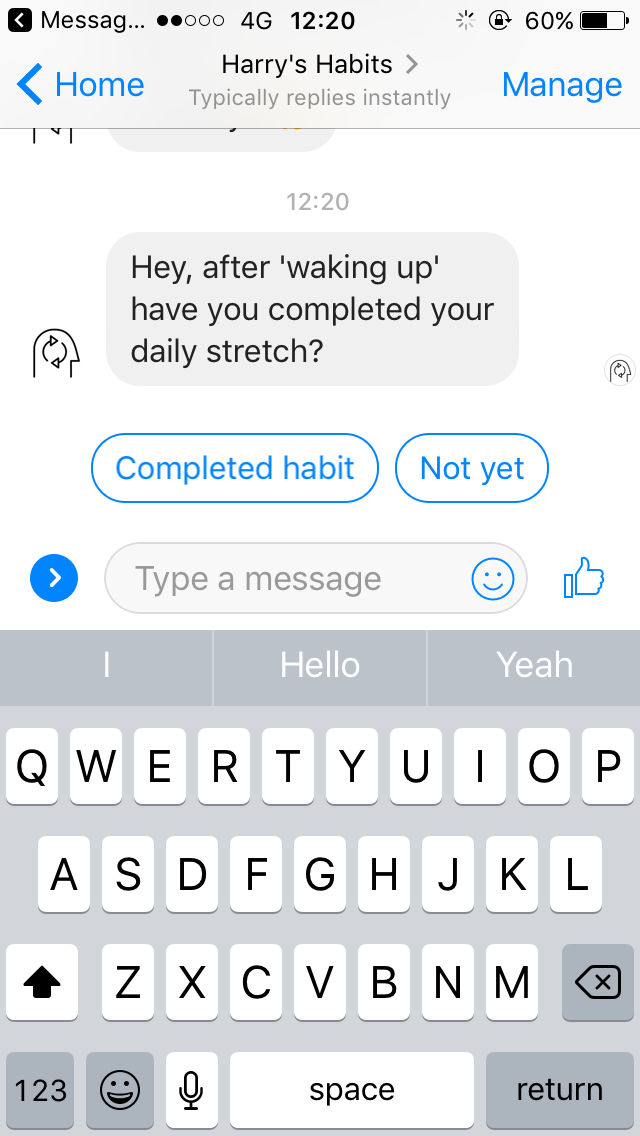
\includegraphics[width=0.47\columnwidth]{figures/reminder.png}
  \hspace{5px}
  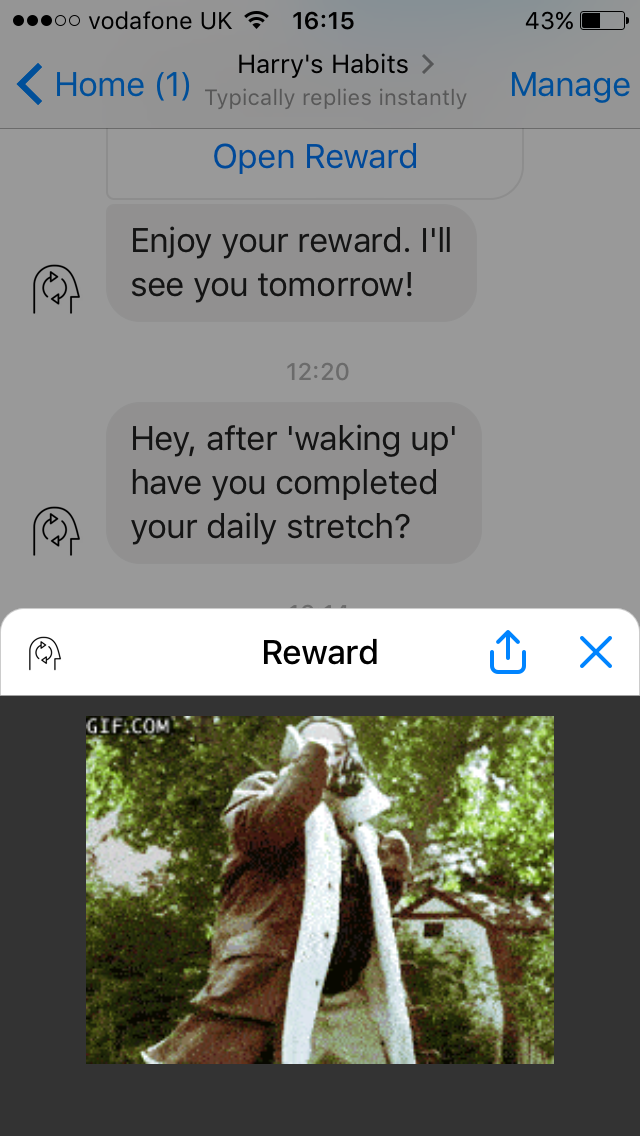
\includegraphics[width=0.47\columnwidth]{figures/reward-visual.png}
  \caption{Bot's ``check in'' message (left) and an example of a reward (right).}~\label{fig:setup}
\end{figure}

\section{Comparing Different Types Of Positive Reinforcement}
The aim of the study was to explore what type of positive reinforcement would be the most effective in supporting regular habit completion and the development of automaticity. We conducted a 4-week situated study followed by semi-structured interviews to evaluate each reward from a different mode using a chatbot to deliver each reward. The study and the bot are described below.

\subsection{Method}
For the purpose of the study, we developed a chatbot that was used to deliver positive reinforcement to participants wanting to start a new healthy habit. To ensure that participants were motivated to pursue their habit, we gave them a choice: they could select one of physical activity habits (stretching, press ups, the plank) or relaxation habits (reading, writing, meditation). We selected these specific habits, as they are easy to complete and generally do not require any special equipment. Moreover, simple tasks become automatic quicker than complex actions~\cite{article_how_habits_formed_modelling_habit_formation} and such simple habits allow to observe changes in automaticity of behaviour within four weeks~\cite{article_beyond_self_tracking_designing_apps}.

\subsubsection{Participants}
Sixty participants were recruited on social networks. They were 18-63 years old (mean age=26.7 years old, SD=10), thirty-five or 58\% were male, fifteen or 25\% were female, ten, 17\% chose not to say, eighteen, or 30\% were university students. Twenty-five participants used a web browser, eighteen used iOS devices, twelve used Android and five used other mobile devices to interact with the bot. Fifteen participants selected meditation, fourteen selected stretch, thirteen selected press ups, six selected reading, five selected writing and seven selected the plank.

\subsubsection{Design}
The participants were randomly assigned to one of four conditions: Audio, Visual, Audio-Visual and the Control group. Each condition differed by the type of positive reinforcement provided to participants: in the Audio condition they received a 15-second audio clip as a reward for completing their habit; in the Visual condition they received a fifteen-second GIF; the Audio-Visual condition combined the audio clip with a GIF; and participants in the Control group received a simple acknowledgement. 

The aim of the rewards was to motivate the participants to keep coming back every day and completing their habits. We identified several ``motivational'' GIFs and audio files, and each GIF file was tweaked to match the audio frequency.


For each condition, we measured the number of times the selected habit was completed during the study (``habit completion'') and the change in automaticity of the behaviour during the final weeks. 

\begin{table}
  \centering
  \begin{tabular}{l l l}
    % \toprule
    {\small\textit{Condition}} & {\small \textit{No. Participants}} & {\small \textit{Positive reinforcement}} \\
    \midrule
    Audio & 15 & 15s audio\\
    Visual & 15 & 15s GIF \\
    Audio-Visual & 15 & 15s GIF and audio \\
    None (control group) & 15 & Confirmation message \\
    % \bottomrule
  \end{tabular}
  \caption{Study conditions and their corresponding types of positive reinforcement}~\label{fig:precise_rewards}
\end{table}

\subsubsection{Materials}
To deliver different types of positive reinforcement, we built a custom Facebook Messenger bot (see Figure~\ref{fig:setup}). Bot's functionality and approach to support habit formation was informed by~\cite{article_beyond_self_tracking_designing_apps}: rather than providing reminders, the bot first allowed participants to define a routine and during the study provided ``check in'' notifications to see if the routine was followed; if the routine was not working and participants did not complete their habit on time, the bot then suggested changes to the plan.

We decided to use a bot as it can easily send notifications, is cross-platform and thus highly available, and also offers simple user interface and easy interactions already familiar to the users. Moreover, the integration with the platform meant that interactions with the bot would be visible alongside participant's other conversations, making it easier to report completion of the habit~\cite{the_power_of_logging_mobile_notifications}.

For the GIF rewards, we decided to use popular internet memes, i.e. content that is passed along from person to person via social media posts~\cite{meme_definition}. Humorous GIF memes make people laugh and are popular on some social media sites, where they usually are the most engaging content~\cite{meme_gifs_are_good}. Given that our bot was integrated with Facebook, and that Facebook introduced built-in support for animated GIFs~\cite{fb_gif_rollout}, memes would integrate well with the bot environment. 

We also used the bot to collect responses to the Self-Report Behavioural Automaticity Index (SRBAI;~\cite{article_4q_SRBAI}). This is a validated 4-item instrument for measuring habit automaticity, which can be used as an indicator of habit strength. SRBA statements are presented on a 5-point Likert scale with answers from 'Strongly Disagree' (1) to 'Strongly Agree' (5); higher scores indicate higher self-reported levels of automaticity.

Information about how well a participant was performing was not revealed, to separate the rewards from other types of motivation, as streaks can provide motivation~\cite{article_dont_kick_habit}. 



\begin{figure}
  \centering
  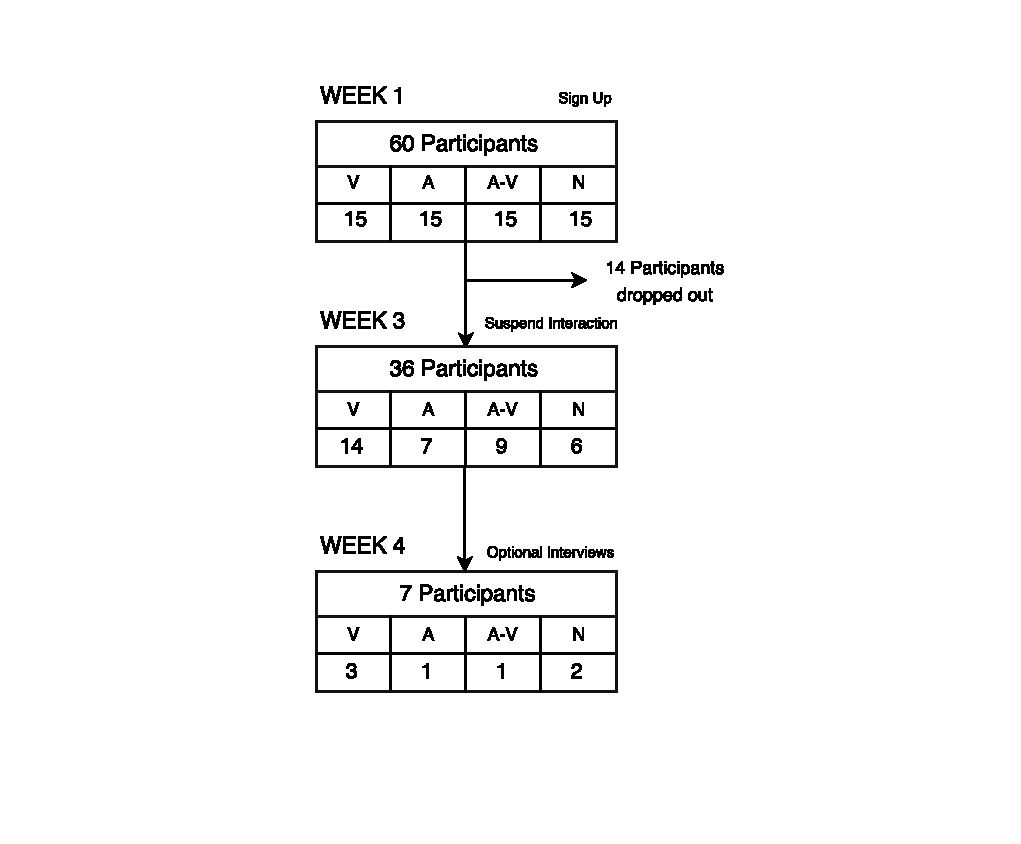
\includegraphics[width=.95\columnwidth]{figures/study-flow.pdf}
  \caption{Participant drop-out during the 4-week study. A: audio, V: visual, A-V: audio-visual, N: no rewards.}~\label{fig:study_dropout}
\end{figure}

\subsubsection{Procedure}
Recruitment posts instructed potential participants to connect with our bot via Facebook Messenger. By connecting with the bot, completing the set-up and providing demographics information, participants expressed their consent to participate in the study.

During the set-up process, participants were asked to select one of the healthy habits they would like to develop and, as recommended in~\cite{article_dont_forget_your_pill} for technologies supporting habit formation, to specify contextual cues associated with that habit and the time they would want to complete it (morning, afternoon, evening). Once their habit routine was specified, participants were automatically assigned to one of the study conditions. 

Next, for the first three weeks of the study, participants were asked to complete their chosen habit as part of the specified routine. During that period, the bot ``checked in'' with the participants after their specified time (see Figure~\ref{fig:precise_rewards}, left). Participants then could indicate whether they completed the habit or not. If they reported habit completion, they would receive their positive reinforcement message (see Figure~\ref{fig:precise_rewards}, right). If they selected ``not yet'', the bot would check on the participant again an hour later. This allowed for the checks to be snoozed, to ensure the new habit fits into participant's routine. If participants constantly told the bot they had not completed their habit yet, the bot would suggest making changes to the routine.

After interacting with the bot for three weeks, participants were asked to complete the SRBAI questionnaire and answer a set of questions about the positive reinforcement they received. Next, during the final week of the study, bot interactions were suspended, but participants were still asked to continue with their habit. At the end of that period, participants were asked to complete the SRBAI questionnaire again along with a few questions about their experience with the reward. Participants also had an option to opt-in for an interview to discuss their experience. The interviews were conducted the after the 4-week study. The study has been approved by the university Ethics Committee, project ID: 54701.



\subsection{Pilot}
We conducted a pilot with five participants to test the bot and study procedures. The pilot resulted in minor language changes and clarifications to bot messages and study instructions.

\section{Results}
Thirty-six participants completed the 4-week study (see Figure~\ref{fig:study_dropout}); seven of them were from the Audio condition, fourteen from the Visual condition, nine were from Audio-Visual and six from the Control group. They were 18-63 years old (mean=27 years old, SD=12), twenty-three (64\%) were male, eleven (30\%) were female and two (6\%) didn't say. 

% Meditation was the most popular habit chosen (twelve participants, or 33\%), followed by press ups (eight participants 22\%), then Stretching (six participants 15\%). Reading and writing were the least, only selected by four and two participants respectively. [how does it compare to the initial list of participants and the habits they selected?]

% Fourteen participants (23\%) dropped out of the study at various stages (Figure~\ref{fig:study_dropout}): fifty-four participants (90\%) continued interacting with the bot and started the set-up. Thirty-nine participants (65\%) completed the set-up and out of these, three participants just ignored all messages from the bot during the trial.  <-- \emph{I don't understand this, numbers don't add up. You say that 60 started the study, but also that 39 completed the set-up. Wasn't completing the set-up the starting point of the study??}

  %Leaving 36 participants (66\%) that are considered active throughout and are included in the final analysis. These 36 participants are 1 36 participants sent a total of 1.1k messages to the bot (mean = 65 messages per participant) and the bot sent 2.7k total messages back. 184 total habits were marked as completed, with the bot issuing 69 visual rewards, 58 audio-visual rewards and 17 audio rewards to those participants. The control group completed 40 habits and were sent 0 rewards.



\subsection{Habit Completion}
Analysis of each individual reward on habit completion (Figure~\ref{fig:m1_h1_a}) revealed that there was a statistically significant difference between each reward as determined by one-way ANOVA ($F(2,624) = 27.007$, $p < 0.05$). A Tukey post hoc test revealed that the difference in completed habits was statistically significantly lower for the audio ($0.081 + 0.274$, $p < 0.005$) and audio-visual ($0.267$ + $0.484$, $p = 0.025$) feedback compared to the visual feedback ($0.373$ + $0.484$).


%Comparing the number of participants who dropped out of the study versus their reward modality, shows that 7 participants who blocked the bot had 27 visual rewards in total (mean = 3.85). 2 participants had 4 total audio rewards (mean = 2) and 2 participants had 2 audio-visual combined (mean = 6.5). These audio-visual participants that dropped out had the highest amount of snoozes (24 total snoozes, 6 and 18 individually, mean = 12), compared with visual 10 total (mean = 2), and audio with 0 snoozes.

% [this section needs cleaning up]

% Stretching (6 participants 15\%) was the most completed habit based on selection (60 times), ranking 10.0 (where 10.0 = 60/6). Meditation ranked 6.25 (6.25 = 75/12) and the least were the plank and reading with 3.75 (15/4) and 1.75 (7/4) respectively.

% Participants (14 participants 39\%) with visual rewards had the highest total number of snoozes (72 total presses to 'Not Yet'), audio had the smallest (14 total). The control group had 55 snoozes and audio-visual had 45 snoozes. Most participants snoozed (answered 'Not Yet') in the morning (100 times), specifically mid (66) and late (27) morning. audio-visual had the most number of failed snoozes (10, split over 6 participants, 1 person had 5 failed snoozes). Then it was audio by 4.

% Habit performance was also tracked in the form of a streak. If a participant did not track a habit for a day, their streak would be reset to 0. Meditation had the most cumulative streak (17) followed by stretching (7). High streaks (streak > 10) had habits: meditation (135 streaks) and stretch (126 streaks). audio-visual rewards had the most streaks (126), control group (75) and visual (60). Stretch had the highest peak streak (18), meditation (15). However, overall, for all completed habits, meditation was the most streaked (269), stretching (231), press ups (39) and plank (24).


\subsubsection{The rewards effect on habit completion}
To explore the effect of rewards on the number of habits completed, compared with the control group, a one-way between-groups analysis of variance with planned comparisons was conducted. Participants were divided into two groups: group 1 with rewards, group 2 without rewards. There was a statistically significant difference at the $p$ $<$ $0.005$ level in both groups for week one and three: week 1, $F(1,23.20) = 9.48$, $p = 0.005$, week 2, $F(1,33.35) = 4.46$, p = 0.42 and week 3, $F(1,50) = 17.01$, $p\leq 0.005$. The effect size for week 1, week 2 and week 3 are large, calculated using $\eta^{2}$, were 0.25, 0.39 and 0.43 respectively, reporting a large difference in the mean scores.

\subsubsection{Audio-visual rewards effect on habit completion}
Multiple modes as feedback has been shown to increase task completion rates~\cite{comparing_modalities_effects_of_visual_auditory, benefits_of_audio_visual_1, benefits_of_audio_visual_2}. However, the results from our study report a significant \textit{decrease} in habit completion for multiple modes (audio-visual). The significance of this finding was tested by conducting a one-way between-groups analysis of variance with planned comparisons (Figure~\ref{fig:m1_h2}). Participants were divided into two groups according to their mode: group 1: audio rewards and visual rewards, group 2: audio-visual rewards. There was a statistically significant  between groups each week ($p$ $<$ $0.005$) Week 1, $F(1,50) = 0.69$, $p = 0.410$, week 2, $F(1,50) = 23.04$, $p$ $<$ $0.005$ and week 3, $F(1,50) = 8.85$. The effect size for week 1, week 2 and week 3 are large, calculated using $\eta^{2}$, were 0.25, 0.39 and 0.43 respectively, reporting an increasing difference in the mean scores throughout weeks.



\begin{figure}
\centering
 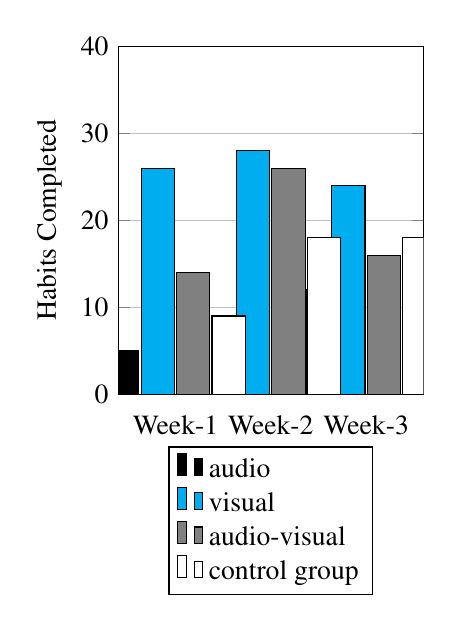
\begin{tikzpicture}
   \begin{axis}[
      width  = 0.45*\textwidth,
      height = 6cm,
      major x tick style = transparent,
      ybar=2*\pgflinewidth,
      bar width=12pt,
      ymajorgrids = true,
      symbolic x coords={Week-1, Week-2, Week-3},
      xtick = data,
      scaled y ticks = false,
      enlarge x limits=0.3,
      ymin=0,
      ymax=40,
      legend cell align=left,
      legend style={at={(0.5,-0.15)},anchor=north},
      ylabel={Habits Completed},
   ]
   
      \addplot[style={fill=black},error bars/.cd, y dir=both, y explicit,error bar style=red]
           coordinates {
          (Week-1, 5)
          (Week-2, 0)
          (Week-3, 12)
           };


      \addplot[style={fill=cyan},error bars/.cd, y dir=both, y explicit]
          coordinates {
          (Week-1, 26)
          (Week-2, 28)
          (Week-3, 24)
          };


      \addplot[style={fill=gray},error bars/.cd, y dir=both, y explicit,error bar style=red]
           coordinates { 
          (Week-1, 14)
          (Week-2, 26)
          (Week-3, 16)
           };
           
      \addplot[style={fill=white},error bars/.cd, y dir=both, y explicit,error bar style=red]
           coordinates { 
          (Week-1, 9)
          (Week-2, 18)
          (Week-3, 18)
           };
      \legend{audio, visual, audio-visual, control group}

  \end{axis}
  \end{tikzpicture}
  \caption{The number of habits completed for each reward over the 3-week period.}~\label{fig:m1_h1_a}
\end{figure}


% \begin{figure}
%   \centering
%  \begin{tikzpicture}
%    \begin{axis}[
%       width  = 0.4*\textwidth,
%       height = 6cm,
%       major x tick style = transparent,
%       ybar=2*\pgflinewidth,
%       bar width=15pt,
%       ymajorgrids = true,
%       symbolic x coords={Week-1, Week-2, Week-3},
%       xtick = data,
%       scaled y ticks = false,
%       enlarge x limits=0.45,
%       ymin=0,
%       ymax=22,
%       legend cell align=left,
%       legend style={at={(0.5,-0.15)},anchor=north},
%       ylabel={Habits Completed},
%    ]
%       \addplot[style={fill=white},error bars/.cd, y dir=both, y explicit]
%           coordinates { % Control group
%           (Week-1, 19)
%           (Week-2, 6)
%           (Week-3, 3)
%           };

%       \addplot[style={fill=black},error bars/.cd, y dir=both, y explicit,error bar style=red]
%            coordinates { % Rewards
%           (Week-1, 21)
%           (Week-2, 16)
%           (Week-3, 18)
%            };

%       \legend{Control, Rewards}

%   \end{axis}
%   \end{tikzpicture}
%   \caption{The effect of positive reinforcement rewards on habit completion.}~\label{fig:m1_h1}
% \end{figure}


\subsection{Habit Completion Discussion}
The results found that participants are more likely to complete their habit if given one of the rewards, especially if the reward was visual. Participants completed more habits with visual rewards than audio rewards or audio-visual rewards.

\subsubsection{Rewards improve habit completion}
There was a statistically significant drop in habit completion for the control group without rewards. This reveals the effect the rewards had on participant interaction with the bot and habit completion. The findings show that rewards did significantly increased habit completion.

\subsubsection{The visual rewards increase habit completion}
There is a significant difference between the audio-visual modes on the number of completed habits. But the result appears to be different to the initial hypotheses, with more participants completing habits with audio rewards and visual rewards than audio-visual. This contradicts existing literature reporting feedback from multiple modes benefits task completion, however these findings are only impacted by the rewards used in this study delivered by the bot. Therefore, it is inconclusive whether audio-visual rewards in a general sense decrease habit completion and visual rewards increase habit completion.

\subsection{Limitations and Future work for Habit Completion}
This research relies on participants self-reporting and participants could have lied to remove the alert instead of performing the habit, just to get the reward. This is particularly true with the snooze function, as the voluntary interviews report that some participants found the bot annoying and stopped using it over time. These participants could have been simply getting rid of the check-in notification rather than completing the habit changing the measurement to how participants reacted to these check-in notifications, instead of their habit. Therefore, it is difficult to draw any valid conclusion on actual habit performance. Future work into how quickly participants responded to the alerts and if the device delivery (browser or smartphone) would better understand how participants interacted with the alerts.

\begin{figure}
  \centering
 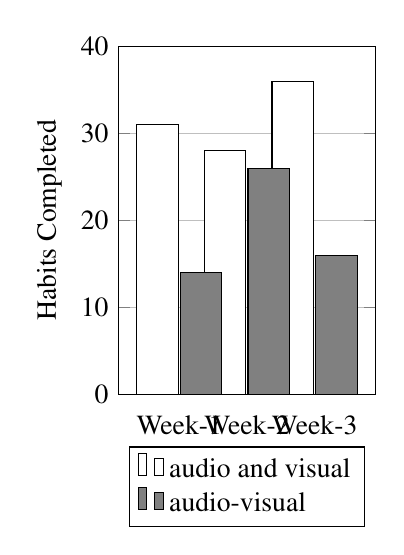
\begin{tikzpicture}
   \begin{axis}[
      width  = 0.4*\textwidth,
      height = 6cm,
      major x tick style = transparent,
      ybar=2*\pgflinewidth,
      bar width=15pt,
      ymajorgrids = true,
      symbolic x coords={Week-1, Week-2, Week-3},
      xtick = data,
      scaled y ticks = false,
      enlarge x limits=0.45,
      ymin=0,
      ymax=40,
      legend cell align=left,
      legend style={at={(0.5,-0.15)},anchor=north},
      ylabel={Habits Completed},
   ]
      \addplot[style={fill=white},error bars/.cd, y dir=both, y explicit,error bar style=red]
           coordinates { % Singular Modes
          (Week-1, 31)
          (Week-2, 28)
          (Week-3, 36)
           };

      \addplot[style={fill=gray},error bars/.cd, y dir=both, y explicit]
          coordinates { % Multiple Modes
          (Week-1, 14)
          (Week-2, 26)
          (Week-3, 16)
          };

   
      \legend{audio and visual, audio-visual}

  \end{axis}
  \end{tikzpicture}
  \caption{The rewards effect on habit completion: audio-visual compared with audio rewards and visual rewards.}~\label{fig:m1_h2}
\end{figure}

\subsection{Habit Automaticity}
The two SRBAI questionnaires, presented in week three and four, are analysed to find out if habit automaticity was built just by using the bot. Eleven participants completed both SRBAI questionnaires: two had the audio condition, five visual, two audio-visual and two were in the control group. A paired-samples t-test was conducted on both questionnaires reporting a statistically significant increase in automaticity scores from SRBAI 1 (mean = 14.18, SD = 3.78) to SRBAI 2 (mean = 15.09, SD = 4.34), $t(10) = 2.469$, $p$ $<$ $0.005$ (two-tailed). Participants habit automaticity did generally increase, as reported by a mean increase in SRBAI scores of 0.90 (CI = 95\%, from 0.08 to 1.72) and a large effect size as measured by $\eta^{2} = 0.37$.

\subsubsection{The rewards effect on habit automaticity}
Comparing participants SRBAI results with the control group shows the impact rewards had on automaticity.
An independent-samples t-test was conducted to compare both SRBAI 1 and SRBAI 2 for rewards and control (Figure~\ref{fig:m2_h1}). For SRBAI 1, there was also no significant differences in scores for rewards (mean = 14.33, SD = 3.84) and control (mean = 13.50, SD = 4.94; $t(9) = 0.224$, $p = 0.85$,
two-tailed). The magnitude of the differences in the means (mean difference = 0.83,
95\% CI: \-29.43 to 27.76) was very small ($\eta^{2} = 0.005$). For SRBAI 2, there was no significant difference in scores for rewards
(mean = 15.22, SD = 4.29) and control (mean = 14.50, SD = 6.36; $t(9) = 0.202$, $p = 0.84$,
two-tailed). The magnitude of the differences in the means (mean difference = 0.72,
95\% CI: \-8.80 to 7.36) was very small ($\eta^{2} = 0.004$). Another test was conducted to validate this finding. A one-way between-groups analysis of variance with planned comparisons was also conducted, but there was not a statistically significant difference for the two groups at SRBAI 1: $F(1,9) = 0.02$, $p = 0.88$, and SRBAI 2: $F(1,9) = 0.07$, $p = 0.78$. In addition, the difference in mean scores between the groups had, at SRBAI 1: a medium effect with an effect size $\eta^{2} = 0.11$, and at SRBAI 2: a large effect, with an effect size of $\eta^{2} = 0.17$.

%       S1 Mean S2 Mean S1 SD   S2 SD
% Control 13.5  14.5  4.949747468 6.363961031
% Rewards 14.33 15.22 3.840572874 4.294699576

\begin{figure}
  \centering
 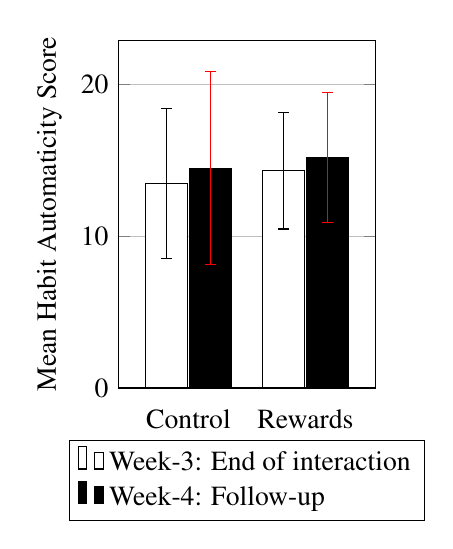
\begin{tikzpicture}
   \begin{axis}[
      width  = 0.4*\textwidth,
      height = 6cm,
      major x tick style = transparent,
      ybar=2*\pgflinewidth,
      bar width=15pt,
      ymajorgrids = true,
      symbolic x coords={Control,Rewards},
      xtick = data,
      scaled y ticks = false,
      enlarge x limits=0.60,
      ymin=0,
      legend cell align=left,
      legend style={at={(0.5,-0.15)},anchor=north},
%       x label style={at={(axis description cs:0.5,-0.1)},anchor=north},
%       y label style={at={(axis description cs:-0.1,.5)},rotate=90,anchor=south},
%       xlabel={$u$ unemployment},
      ylabel={Mean Habit Automaticity Score},
   ]
      \addplot[style={fill=white},error bars/.cd, y dir=both, y explicit]
          coordinates {
          (Control, 13.5) += (0,4.94) -= (0,4.94)
          (Rewards, 14.33) += (0,3.84) -= (0,3.84)
          };

      \addplot[style={fill=black},error bars/.cd, y dir=both, y explicit,error bar style=red]
           coordinates {
           (Control, 14.5) += (0,6.36) -= (0,6.36)
           (Rewards, 15.22) += (0,4.29) -= (0,4.29)
           };

      \legend{Week-3: End of interaction, Week-4: Follow-up}

  \end{axis}
  \end{tikzpicture}
  \caption{The rewards effect on habit automaticity. Comparing mean habit automaticity for rewards versus control group.}~\label{fig:m2_h1}
\end{figure}

\subsubsection{Audio-Visual versus Audio, Visual modes on habit automaticity}
To compare the effect audio-visual had on automaticity a one-way between-groups analysis of variance with planned comparisons was conducted (Figure~\ref{fig:m2_h2}). Participants were divided into two groups according to their reward mode: group 1: audio rewards and visual rewards and group 2: audio-visual rewards. There was not a
statistically significant difference for the two groups at SRBAI 1: $ F(1,9) = 1.04$, $p = 0.33$, and SRBAI 2: $F(1,9) = 0.64$, $p = 0.44$. In addition, the difference in mean scores between the groups had, at SRBAI 1: a medium effect with an effect size of $\eta^{2} = 0.11$, and at SRBAI 2: a large effect, with an effect size of $\eta^{2} = 0.17$.




%       S1 Mean S2 Mean S1 SD S2 SD
% Visual  14.6  15.8  4.336 3.701
% audio  12    11.5  4.243 6.364
% V-A   16    17.5  2.828 3.536

\begin{figure}
  \centering
 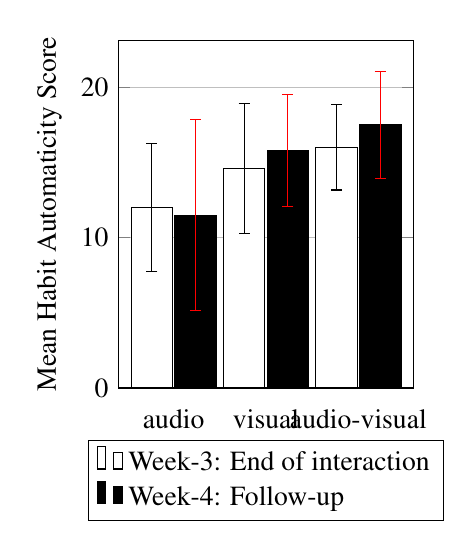
\begin{tikzpicture}
   \begin{axis}[
      width  = 0.44*\textwidth,
      height = 6cm,
      major x tick style = transparent,
      ybar=2*\pgflinewidth,
      bar width=15pt,
      ymajorgrids = true,
      symbolic x coords={audio, visual, audio-visual},
      xtick = data,
      scaled y ticks = false,
      enlarge x limits=0.3, % how far apart the bars are
      ymin=0,
      legend cell align=left,
      legend style={at={(0.5,-0.15)},anchor=north},
%       x label style={at={(axis description cs:0.5,-0.1)},anchor=north},
%       y label style={at={(axis description cs:-0.1,.5)},rotate=90,anchor=south},
%       xlabel={$u$ unemployment},
      ylabel={Mean Habit Automaticity Score},
   ]
      \addplot[style={fill=white},error bars/.cd, y dir=both, y explicit]
          coordinates {
          (audio, 12) += (0,4.243) -= (0,4.243)
          (visual, 14.6) += (0,4.336) -= (0,4.336)
          (audio-visual, 16) += (0,2.828) -= (0,2.828)
          };

      \addplot[style={fill=black},error bars/.cd, y dir=both, y explicit,error bar style=red]
           coordinates {
          (audio, 11.5) += (0,6.364) -= (0,6.364)
          (visual, 15.8) += (0,3.701) -= (0,3.701)
          (audio-visual, 17.5) += (0,3.536) -= (0,3.536)
           };

      \legend{Week-3: End of interaction, Week-4: Follow-up}

  \end{axis}
  \end{tikzpicture}
  \caption{Audio-Visual versus audio rewards and visual rewards on habit automaticity. Comparing mean habit automaticity for each group.}~\label{fig:m2_h2}
\end{figure}

\subsection{Interview Feedback}
Seven interviews with participants were conducted to gather their experience with their habit completion after the prototype bot was removed. The interview transcripts were analysed and participants were anonymised following a thematic approach~\cite{thematic_analysis_qualatitive_data} \emph{[I dont think I actually did this.]}. Below, we consider the role of each participants during the process of interacting with the chatbot and reflect how their interaction may of had a meaningful impact to their formation of a new habit.

 \emph{[Should I include the full transcripts? I have them im my thesis appendix already written up, if need. - HMT]}
 
\subsubsection{Habit Repetition}
Participants discussed how they picked their habit, they chose because they had wanted to start for the particular habit for a long time, it was \textit{'not too much effort'} and \textit{'something successful people do'}. They wanted \textit{'to be more active'}, \textit{'relieve stress'} and wanted a habit that was \textit{'less time consuming'}. Throughout, participants mostly completed their habits, but, one participant always put the message off and eventually their habit completion got \textit{'worse and worse'} until they stopped all together. This is confirmed after the bot was removed, with all interviewed participants (N = 7) finding it difficult to continue with their habit. They \textit{'kept forgetting'}, found it \textit{'harder to remember'} and lacked motivation, not performing the action if it had \textit{'been a long day'}. Some tried to do it \textit{'every now and again'}, but usually they would only complete it if \textit{'they remembered'}. This reveals the dependency between technology and habits, suggesting that the bot did not increase habit automaticity, or that the existing routine participants chose was not suitable for new habits, or that they were not given enough time to develop automaticity.

\subsubsection{Attitudes Towards Rewards}
Participants had mixed feelings about the rewards. Some \textit{'did not like the [visual] rewards'}, skipping over them after the first few, they \textit{'just wanted to get rid of the notification dot'}. Another participant said \textit{'some of them [audio-visual rewards] were funny'}, but they did not like them overall and mentioned the audio rewards were \textit{'too random'}. One participant thought they did not give them an incentive towards their habit, just a \textit{'nice little extra'}. They also discussed including time-sensitive rewards, as they did not want to listen to music before going to bed. This shows the importance of using an appropriate modality at particular times, e.g. not having audio rewards at certain times of the day. Finally, an upbeat participant talked about \textit{'always wanting to open them'} and \textit{'the combination was perfect'}. However, they said they also found them \textit{'repetitive'} and one participant stated that they simply wanted to get rid of the notification. This implies that the bot was not tracking how many habits that participant completed, but instead tracking how many times that participant wanted the bot to stop messaging them.

\subsubsection{Attitudes Towards the Chatbot}
Participants were asked about how they found the chatbot as the method of interaction. They found the method \textit{'pretty good'}, they \textit{'liked it'} and \textit{'would have liked more interaction'}. Suggesting additional features, such as \textit{'help and support throughout'}, \textit{'ideas on how to improve your habit'} and \textit{'advice on how to set aside time for your habit'}. Others were neutral, some expecting \textit{'different messages, such as Hey [name], a bit more care about the person, a bit less like a robot'}. Four participants enjoyed the back up notification aspect, but a few found it \textit{'repetitive'} and \textit{'got annoying if I pressed Not Yet'}. Participants wanted to see their progress as they tracked their habits, they talked about wanting to reflect on their data. They mentioned that they would feel \textit{'more encouraged to keep doing it, rather than random music [audio rewards]'}. Mostly participants wanted the prototype to come back with a few modifications: \textit{'enclosed with Fitbit so it is all in a single place'}, \textit{'fine without rewards'} (2 participants mentioned this), \textit{'more interaction'} and \textit{'with statistics about my progress'}. Participants wanted the bot as more of a \textit{'constant persistent reminder'} with additional tracking elements to remind them to perform their habit to fit into their busy schedule. Participants (N = 5) mentioned the \textit{headspace} app (\url{www.headspace.com}), mentioning that they wanted a combination of the bot and headspace. It prompted another participant to download the headspace app. They wanted the bot to keep on track of their habit and they would use the headspace app to help them perform their mindfulness.

\subsubsection{Summary}
Participants picked habits they wanted to perform, but when the bot stopped notifying them, they lacked motivation to completed their habit. Some participants enjoyed the rewards at the beginning, but most participants disliked them after the first week.

\subsection{Habit Automaticity Discussion}
It is inconclusive whether the rewards or the combined modalities effected habit automaticity. 

% \subsubsection{The Rewards effect on Habit Automaticity}
Each individual reward did not have a significant effect on habit automaticity. Although participants with rewards had slightly higher automaticity scores and follow up interviews suggest that automaticity did not develop with participants discussing negative feelings towards rewards during the interviews.  

% \subsubsection{M2H2: Multiple Modalities effect on Habit Automaticity}
Participants with audio-visual rewards had higher habit automaticity scores compared with audio or visual rewards. However, this difference was not statistically significant.

\subsection{Limitations and Future work for Habit Automaticity}
Only seven participants responded to the follow up interviews. In addition, the study relied on participants recall which could be inaccurate. Future work conducting similar research with a larger sample size for the SRBAI questionnaire would validate these findings

\section{General Discussion}
This research aimed to understand more about rewards from different modalities and their role in habit formation. Participants receiving bot-delivered rewards completed more habits than the control group without rewards. There was a significant correlation between the habit formation method and habit automaticity. However, this was contradicted during the participant interviews where all seven participants reported a drop in habit completion after 1-week without the prototype.

% Under half the participants completed the modality survey (N = 12, 40\%). These had the following rewards: visual rewards had the highest score (the higher, the more participants preferred the reward) (mean = 12, SD = 3.347), visual and audio rewards were slightly below (mean = 10.75, SD = 1.893).
% TODO: Compare these results to people not using the chatbot, e.g.. people signing up to the gym, new years resolution

\subsection{Prototype Success}
The chatbot was partially successful at running a research trial. There were several issues and various limitations with development. However, it was generally liked by participants and it was easy to gather a lot of useful data.

Participants had mixed feelings towards the bot. Their performance shows that the number of snoozes over time decreased, but the number of total habits completed per day also decreased for all reward types (including the control group). However, participant streaks over time increased and 36 participants manage to use it for 3-weeks.

Participants had various issues with bot interaction. Seven participants tried to message the bot during setup, instead of using the built in \textit{quick reply} buttons. This broke the setup flow and they had to start again. Other participants tried to send multiple messages when asked for free input, they went around an endless loop when asking for a habit type and participants tried to mark their habit as completed using the Facebook Messenger thumb emotion (which the bot was not coded for). A participant also pointed out that they could change their existing routine time but were unable to change the description.

Participants gave additional feedback by simply messaging the bot. They asked inquisitive questions, such as \textit{'what kind of thing are you looking to find out'}, \textit{'this is not working for me'} and \textit{'stop'} --- to try and stop the daily messages (the participant then blocked the bot). Negative feedback towards the rewards and bot were also expressed. When asked about being messaged every day, a participant sent this reply and then blocked the bot: \textit{'Do not do that, it will be annoying'}, and another said \textit{'never message me'}. Another stated that this was the \textit{'lame same band'} after receiving an audio reward.

Participants were able to personalise the chatbot with several different variable configurations. This personalisation could have effected the findings by not narrowing the condition variables. Replicating this research with tighter a configuration is needed to validate this line of reasoning. Finally, streaks could have been better used to give insight to participants progress and challenged them to maintain it, using loss aversion~\cite{loss_aversion} to compare the impact of their broken streak with the gain of keeping it. However, all participants interviewed (N = 7) struggled with maintaining habit completion after the bot was removed. This suggests a dependence between the technology and the habit as participants depended on bot notifications to continue repeating the desired action.

The chatbot rewards from different modalities effected habit formation with the singular modes improving habit completion, but not habit automaticity. Feedback towards interaction with the chatbot was mostly positive, but all interviewed participants suggested features they would like, likely because it did not fulfil their needs. The rewards delivered by the chatbot got a mixed reception from participants and did not significantly increase habit automaticity, but they did improve the number of habits participants completed. Therefore, the chatbot is partially effective for supporting habit formation.

% \subsection{Dependence}
% Streaks could have been better used to give insight to participants progress and challenged them to maintain it, using loss aversion~\cite{loss_aversion} to compare the impact of their broken streak with the gain of keeping it. However, all seven participants interviewed struggled with maintaining habit performance after the bot was removed. This suggests a dependence between the technology and the habit as participants depended on bot notifications to continue repeating the desired action.

\subsection{General Limitations and Future Work}
This research has four key limitations. First, the small number of participants and the small sample of rewards used in the study make it unclear how these findings would generalise to other types of rewards with the same modality. Second, these findings only apply to intrinsic positive reinforcement rewards and further research into using different types of rewards as positive reinforcement is needed.  Finally, the content and method of delivery is another variable that effects these results and additional studies into the effect of bot-delivered rewards on habit formation would validate these findings. 

\section{Conclusions}
The results found that the rewards did not impact habit automaticity, but it increased generally, while using the bot. However, the rewards did improve the number of habits people completed, with the highest completion rates for visual rewards. Habit completion was also affected by the different modalities, although not in the way our hypotheses assumed. Audio-visual rewards had the lowest habit completion when compared with the others. Finally, the limitations of the study do not show any clear statistical significance whether the audio and visual rewards affected habit automaticity. More conclusive evidence is needed to show that rewards from combined modalities effect habit formation. We hope this research opens up new avenues for using bots as tools to help form new habits and give new behaviour change technology insights into positive reinforcement rewards from audio, visual and audio-visual modalities.

% -- FINDINGS --
% AUTOMATICITY
% Bot increased automaticity
% Specific rewards didn't increase automaticity

% COMPLETION
% Visual rewards then audio had highest completion increase
% Audio-Visual rewards actually decreased completion

\section{Acknowledgements}
Thank you to all the participants involved, the internal reviewers and staff who provided helpful feedback throughout the study.

\balance{}

% % Either:
% %  1. Put \balance in the first column of the last page
% %  2. Don't use \balance
% %  3. hard-code a column break into the bbl file (before submission)
% % see more http://stackoverflow.com/questions/2149854/how-to-manually-equalize-columns-in-an-ieee-paper-if-using-bibtex
% \balance{}


\bibliographystyle{scaffold/SIGCHI-Reference-Format}
\bibliography{sample}

\end{document}
